\documentclass{sigchi}

\usepackage[utf8]{inputenc} % for a UTF8 editor only
\usepackage{biblatex}
% Load basic packages
\usepackage{balance}       % to better equalize the last page
\usepackage{graphics}      % for EPS, load graphicx instead 
\usepackage[T1]{fontenc}   % for umlauts and other diaeresis
\usepackage{txfonts}
\usepackage{mathptmx}
\usepackage[pdflang={en-US},pdftex]{hyperref}
\usepackage{color}
\usepackage{booktabs}
\usepackage{float}
\usepackage{textcomp}
\usepackage{tikz}
\usetikzlibrary{shapes, arrows}
\addbibresource{references.bib}


% Some optional stuff you might like/need.
\usepackage{microtype}        % Improved Tracking and Kerning
% \usepackage[all]{hypcap}    % Fixes bug in hyperref caption linking
\usepackage{ccicons}          % Cite your images correctly!

% If you want to use todo notes, marginpars etc. during creation of
% your draft document, you have to enable the "chi_draft" option for
% the document class. To do this, change the very first line to:
% "\documentclass[chi_draft]{sigchi}". You can then place todo notes
% by using the "\todo{...}"  command. Make sure to disable the draft
% option again before submitting your final document.
%\usepackage{todonotes}

% Paper metadata (use plain text, for PDF inclusion and later
% re-using, if desired).  Use \emtpyauthor when submitting for review
% so you remain anonymous.
\def\plaintitle{Reddit cryptocurrency comments analysis}
\def\plainauthor{First Author, Second Author, Third Author,
  Fourth Author, Fifth Author, Sixth Author}
\def\emptyauthor{}
\def\plainkeywords{Reddit; Cryptocurrency; Analysis; Bitcoin Price; PageRank; Louvain; Correlation.}
% \def\plaingeneralterms{Documentation, Standardization}

% llt: Define a global style for URLs, rather that the default one
\makeatletter
\def\url@leostyle{%
  \@ifundefined{selectfont}{
    \def\UrlFont{\sf}
  }{
    \def\UrlFont{\small\bf\ttfamily}
  }}
\makeatother
\urlstyle{leo}

% To make various LaTeX processors do the right thing with page size.
\def\pprw{8.5in}
\def\pprh{11in}
\special{papersize=\pprw,\pprh}
\setlength{\paperwidth}{\pprw}
\setlength{\paperheight}{\pprh}
\setlength{\pdfpagewidth}{\pprw}
\setlength{\pdfpageheight}{\pprh}

% Make sure hyperref comes last of your loaded packages, to give it a
% fighting chance of not being over-written, since its job is to
% redefine many LaTeX commands.
\definecolor{linkColor}{RGB}{6,125,233}
\hypersetup{%
  pdftitle={\plaintitle},
% Use \plainauthor for final version.
%  pdfauthor={\plainauthor},
  pdfauthor={\emptyauthor},
  pdfkeywords={\plainkeywords},
  pdfdisplaydoctitle=true, % For Accessibility
  bookmarksnumbered,
  pdfstartview={FitH},
  colorlinks,
  citecolor=black,
  filecolor=black,
  linkcolor=black,
  urlcolor=linkColor,
  breaklinks=true,
  hypertexnames=false
}

\usepackage[inline]{enumitem}
\usepackage{tasks}



% create a shortcut to typeset table headings
% \newcommand\tabhead[1]{\small\textbf{#1}}

% End of preamble. Here it comes the document.
\begin{document}

\title{\plaintitle}

\numberofauthors{3}
\author{%
  \alignauthor{Albin Aliu\\
    % \affaddr{for Submission}\\
    % \affaddr{University of Fribourg}\\
    \email{\href{mailto:albin.aliu@unifr.ch}{\color{black}albin.aliu@unifr.ch}}}\\
  \alignauthor{François-Xavier Wicht\\
    % \affaddr{for Submission}\\
    % \affaddr{University of Fribourg}\\
    \email{\href{mailto:francois-xavier.wicht@unifr.ch}{\color{black}francois-xavier.wicht@unifr.ch}}}\\
      \alignauthor{Grégoire Rebstein\\
    % \affaddr{for Submission}\\
    % \affaddr{University of Fribourg}\\
    \email{\href{mailto:gregoire.rebstein@unifr.ch}{\color{black}gregoire.rebstein@unifr.ch}}}
}

\maketitle

\begin{abstract}
Lorem ipsum dolor sit amet, consectetur adipiscing elit. Aliquam vulputate, eros nec fringilla commodo, arcu libero tristique magna, sed placerat mauris nisl ac quam. Sed sed purus ac eros viverra pharetra ac eget lacus. Suspendisse laoreet condimentum lorem sit amet bibendum. Morbi volutpat lectus vitae massa porttitor sollicitudin. Sed maximus ipsum vel est feugiat luctus. Sed suscipit lorem et est scelerisque gravida. Sed sed leo ac enim feugiat bibendum eu eget purus. Maecenas eget sollicitudin mi. Proin hendrerit luctus leo, ut cursus augue tempor ac. 

\end{abstract}


% ACM Classfication

% \begin{CCSXML}
%   <ccs2012>
%   <concept>
%   <concept_id>10003120.10003121.10003122.10003334</concept_id>
%   <concept_desc>Human-centered computing~User studies</concept_desc>
%   <concept_significance>500</concept_significance>
%   </concept>
%   <concept>
%   <concept_id>10003120.10003130</concept_id>
%   <concept_desc>Human-centered computing~Collaborative and social computing</concept_desc>
%   <concept_significance>300</concept_significance>
%   </concept>
%   </ccs2012>
% \end{CCSXML}

% \ccsdesc[500]{Human-centered computing~User studies}
% \ccsdesc[300]{Human-centered computing~Collaborative and social computing}

% \ccsdesc[500]{Human-centered computing~Human computer interaction (HCI)}
% \ccsdesc[100]{Human-centered computing~User studies}

% Author Keywords
\keywords{\plainkeywords}

% Print the classification codes
% \printccsdesc
% Please use the 2012 Classifiers and see this link to embed them in the text: \url{https://dl.acm.org/ccs/ccs_flat.cfm}
\section{Introduction}
Since the rise of cryptocurrencies, a lot of research have attempted to predict their price rates \cite{kooPredictionBitcoinPrice2021,coccoPredictionsBitcoinPrices2021,liMultiwindowBitcoinPrice2021}. Due to the transparency of cryptocurrency transactions, researchers have considered using transaction information such as overall trends and cyclical changes to predict cryptocurrency prices \cite{liCrossCryptocurrencyRelationship2022}.

In this project, we attempt to find a link between the activity in cryptocurrency subreddits and the price of Bitcoin. For that purpose, we scraped data directly from said subreddits, structured data in a network architecture and performed several analysis such as PageRank, Louvain community detection and correlation analysis.

This report is structured the following way. Firstly, we discuss the scraping methodology we used, secondly the data models we tried and considered for the analysis and thirdly we outline the analysis of our model. As a closing word, we highlight trials and errors during this project.

%\section{Overview}
%Here we give a brief overview of the project.


\section{Data Collection}
Reddit is a social news aggregation composed of different communities called subreddit, where people gather to discuss and comment on a specific subject. Each subreddit is composed of main posts which are in turn commented and voted either positively (upvoted) or negatively (downvoted). Each comment in turn can also be commented and voted upon which sometimes create a cascade of recursive comments as shown on figure \ref{tab:commentstruct}. To capture these information and later work on it, we use the official Reddit API. To facilitate our work, we used the wrapper PRAW (Python Reddit API Wrapper) library.

To facilitate this data collection, we automated periodic calls to the API in form of a bot. Our bot runs on a linux server and checks all 20 minutes for new posts on specific subreddits. For this project, we used the following list of subreddits: Bitcoin, Ethereum, Dogecoin, BitcoinBeginners, CryptoCurrencies, CryptoTechnology, CryptoMarkets, Binance, CoinBase, btc.
Using the multiprocessing package of python, we spawn a process for each subreddit for the scraping to happen in parallel.
Also, since we care about actual and real time data, we consider the following sorting options provided by the Reddit API: hot posts, top posts and new posts. We don't set some time bound on when the post has been published, since we store the timestamps of each post and comment and filter what we need. This works really well and we didnt encounter any API limitations.

Everytime a new scraping run is started, we create a new JSON file with the timestsamp of the start of the scraping. All new posts that will be found in this run, will be stored inside the newly created JSON file. As time goes by, a post might receive many new comments. Therefore, if a previously crawled post has an increase in comments of more than 30\%, we also refetch that post and update the JSON file it was originally stored in. Once we have a certain amount of raw data, we need to preprocess this data and create data models to ease the analysis. This the object of the next section.

\section{Data Models}
Once we have a certain amount of raw data, we need to preprocess this data and create data models for our graph. We opted for four different data models. Not all were used along the way.

\subsection{Unique Cartesian Link}
This is probably the most natural way to create an undirected graph from our data. All we do is: all users that commented on a post get linked together in a complete graph with edge weight 1. If there is already an edge between two users, the weight of the edge gets increased by 1. This creates an enormously large graph compared to our other data models. This makes computation on the graph very difficult and slow. That's why we opted for other models.

\subsection{Deep Link}
In here, we connect each user to the original poster (OP) and to all users who replied to the user's comment. The edges get a weight depending on the depth of the comment and the achieved upvote score. If there is already an edge between the two users, the weight gets increased. This is a directed graph.


%user0 (OP)
% 	- user1 (d=1, score=10)
% 		- user 2 (d=2, score=10)
% 		- user 3 (d=2, score=2)
% 	- user4 (d=1, score=5)
% 	- user5 (d=1, score=3)
% 		- user6 (d=2, score=2)
% 			- user3 (d=3, score=1)
% 		-user 7 (d=2, score=1)

% figure graph_model


\subsection{Next Link}
Same as Deep Link, except that we only connect each user to the OP and the immediate users who commented directly on the user's comment. Also a directed graph.

\subsection{Deep Link No Merge}
The same as Deep Link but here we don't merge the weights and allow multiple edges from one user to another. Thus, this is a directed multigraph. We found that this approach has still lots of information but is not too expensive to compute.












\section{Analysis and Visualisation}
In this section we pursue with the analysis of data scrapped on several cryptocurrency subreddits. More precisely, we use social media analytics on the network that we built in the previous section. Firstly, we investigate if our network follows a power law distribution as it should. Secondly, we discuss the results of the PageRank algorithm on the network. Thirdly, we run Louvain community detection algorithm and compare the results with the existing subreddits. And finally we analyse the price development of the Bitcoin and try to find a correlation with our data.

\subsection{Power Law Distribution}

The power law distribution in a network can be understood as ``a few users are very popular and a lot of users are mildly or not popular at all''. Intuitively, this relation holds in our network composed of vertices as users and edges representing the comment relation. Indeed, when browsing Reddit in general, we may notice that a few comments (users) are very popular (have a very high score) as others are not. This intuition reveals itself true when plotting the node degree distribution (see fig. \ref{fig:degdist}). This is encouraging in relation to our network model and further analysis because natural networks tend to follow that law. It therefore means that our network is properly formed that the analysis that follows is most likely consistent natural laws.
\begin{figure}[H]
    \centering
    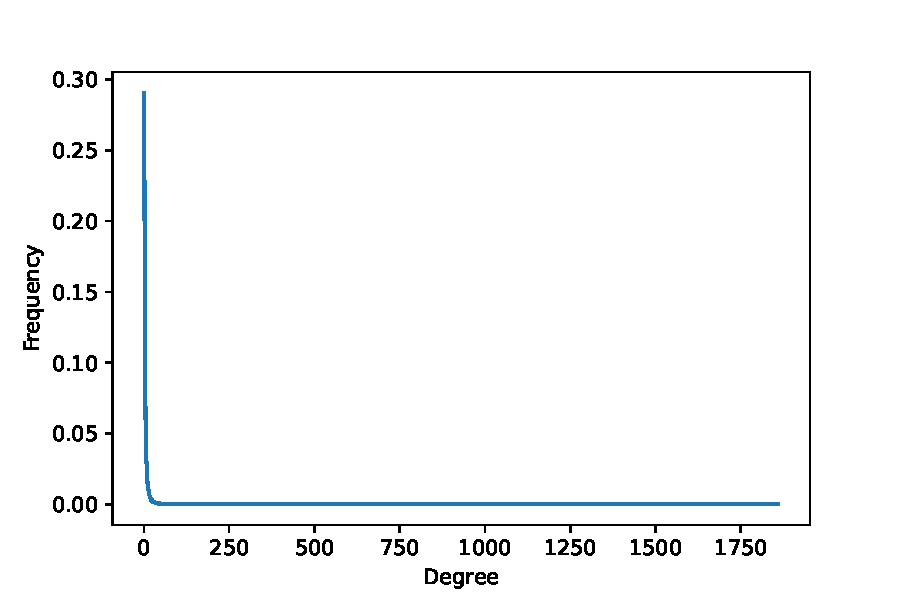
\includegraphics[width=0.3\textwidth]{figures/deg_dist.pdf}
    \caption{The network follows a power law distribution: a lot of users have few comments on their posts and a few users have a lot of comments on their posts.}
    \label{fig:degdist}
\end{figure}



\subsection{Page Rank}

Regarding PageRank (PR), it can be interpreted as the amount of random walks in the network that end up on a particular vertex. For our network, it means that the higher the rank of one user is, the higher the probability is of commenting one post of that particular user. We decide here to investigate the steadiness of PR over 15 days. We might observe unsteadiness on figure \ref{fig:rankdays} but this is not entirely true with respect to the PageRank. First, this is true that the graph evolves quite rapidly over the days. The same users will not necessarily be active twice on the same comment over multiple days. This observation has been done by computing the set of users over the days and devising the similarity for each successive day. Let $U_i$ be the set of users for day $i$, then $s\left(i,j\right)$ is the similarity between day $i$ and $j$ such that $$s\left(i,j\right)=\frac{U_i\cap U_{j}}{U_i\cup U_{j}}.$$ We get the graph at figure \ref{fig:simdays}. However, the PR itself seems to be pretty consistent over the days when we compute the sum of the squared error between the intersected PR values as shown in graph \ref{fig:errordays} where the error only spikes to a value of $0.005$. We can conclude from these two observations that, although there are few overlapping users over the days, the ones that overlap tend to be very popular for a long period. This also means that in the cryptocurrency subreddits, posts tend to have a lasting interest for the users. This conclusion is consistent with the paper \cite{glenskiCharacterizingSpeedScale2019} where they state that cryptocurrencies discussion are likely to trigger a longer lasting discussion.
\begin{figure}[H]
    \centering
    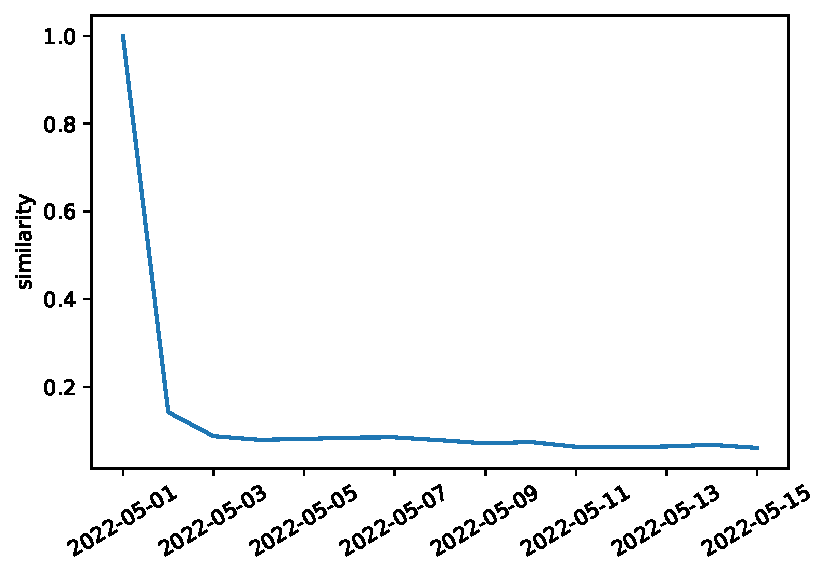
\includegraphics[width=0.3\textwidth]{figures/sim_days.pdf}
    \caption{Similarity between user sets over the 1st to the 15th May.}
    \label{fig:simdays}
\end{figure}
\begin{figure}[H]
    \centering
    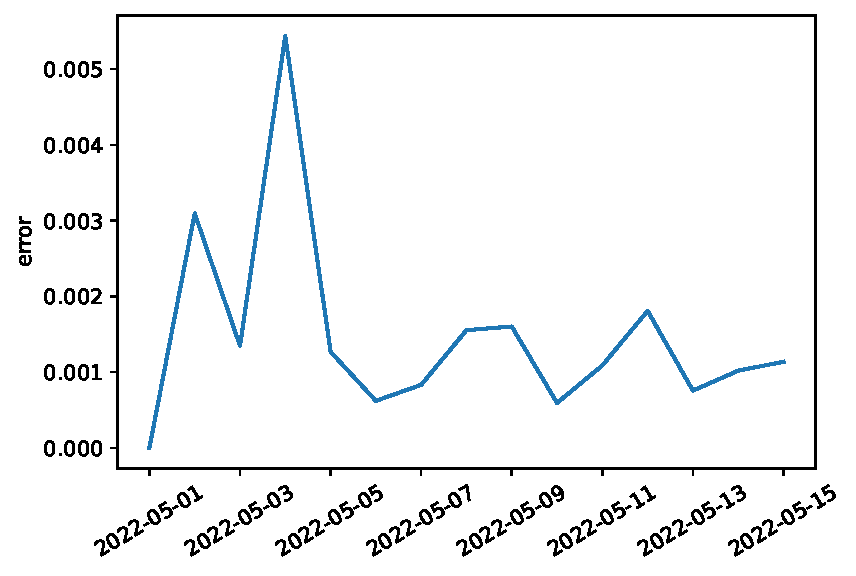
\includegraphics[width=0.3\textwidth]{figures/error_days.pdf}
    \caption{Sum of the squared error of PageRank values over intersected user sets between the 1st and the 15th May.}
    \label{fig:errordays}
\end{figure}

\begin{figure}[H]
    \centering
    \includegraphics[width=0.5\textwidth]{figures/rank_days.pdf}
    \caption{Networks between the 1st to the 15th May. The size of the nodes is relative to the PageRank values.}
    \label{fig:rankdays}
\end{figure}

\subsection{Louvain}
Louvain method is a technique that find communities from large networks. In our case, we were interested to see the communities of our network and observe the links with the different subreddits. To do this, we first create a list of communities corresponding to each subreddit. Each person is assigned to a single community, the one where he/she has interacted the most. Then, we create a second list of communities by applying the Louvain method on the graph based on the \textit{Deep Link No Merge} data model.
After this, we get a list of 260 communities. Knowing that there are 10 subreddits, one subreddit can therefore have several inner communities. 

It can also be interesting to know if some communities are formed by people from different subreddits. For this, we loop over the Louvain communities and compute the percentage of people coming from each subreddit. As a result matrix where rows are Louvain communities and columns are the percentage of people from each subreddit. To have a better understanding of the result, we can plot a histogram of the number of different subreddits that people in a Louvain community belong to (see figure \ref{fig:louvainrepartition}).

\begin{figure}[H]
    \centering
    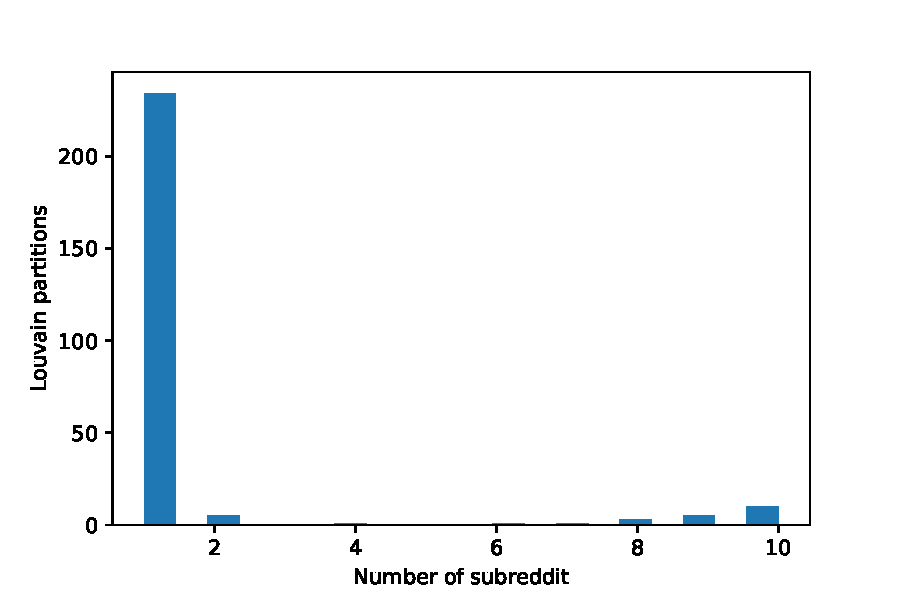
\includegraphics[width=0.3\textwidth]{figures/inner_communities_repartition.pdf}
    \caption{ Repartition of Louvain communities in the subreddits.}
    \label{fig:louvainrepartition}
\end{figure}

With this histogram, we can observe that for the majority, the Louvain communities are formed by people from the same subreddit. However, there is also some Louvain communities that are not restricted to one subreddit but are even made up of people from all 10 subreddits.

\subsection{Correlation to price development}

We wanted to capture the activity of our data. To do so, we group our data by some time window; we chose 1 hour. We create a graph $G_0$ from the first time window. Then we create a second graph $G_1$ from the first union second time window. We continue until we have an inclusion sequence such that 
$$ G_0 \subset G_1 \subset  ... \subset G_{n-1},$$

where $n$ is the number of time windows, and $G_i$ a graph based on the \textit{Deep Link No Merge} data model.
Then, we use the degree centrality to compare each graph with its subsequent graph. This results into a table where we have for each user (node) the development of its activity (degree). With this huge dataset, it is now possible to track users and also identify the most active users. However, since this requires lots of computation power and much more work to get something meaningful from this, we opted for the option to sum each time frame (e.g. 1 hour in our case). 

We're now at that stage where one could run some correlation method on our summed activity dataset against the price data. However, this will not yield good results as both datasets are very volatile. Therefore we needed to smoothen our data somehow. We opted for the moving window average method. We took both datasets and computed moving window averages with step 2, 3, 4, ..., 30. These steps represent the number of columns that will be averaged. 

% figure activity_x_price.pdf 
% figure acvitity_sums_ma.pdf


Then, we compared each activity moving window average for each price moving window average using two of pandas built-in correlation methods, namely Pearson, Spearman and we also tried the The Hilbert–Schmidt independence criterion (HSIC). The first two methods deliver strong correlation coefficients (up to 0.87), while the HISC does not. Also, we notcied that the correlation differs depending on how much days (from when to when) we try to correlate. We've found that more than 10 days usually yields better results. Please refer to the interactive notebook for details.


%% ADDED BY FX AFTER READING CITED PAPER

However, it is important to remember that a correlation between two sets of data does not necessarily indicate a causal link. Here we rely on the results given by paper \citetitle{wooleyExtractingCryptocurrencyPrice2019} and assume that there is a causal link. \citeauthor{wooleyExtractingCryptocurrencyPrice2019} have indeed been able to prove a causal link between price movements and Reddit activity notably with bivariate Granger causality tests. Furthermore, the results shown above are consistent with \citetitle{iderCryptocurrencyReturnPrediction2022} where the authors are able to predict a future price changes with an accuracy significantly better than random guesses \cite{iderCryptocurrencyReturnPrediction2022}.


% figures:
% pearson.pdf
% spearman.pdf
% hisc.pdf




\section{Homemade implementations}
In this section, we discuss the two homemade implementations of the algorithm used in this project: PageRank and Louvain community detection.

PageRank is an iterative process that can potentially last forever. As a stopping condition we put a number of iterations as well as an error threshold. If the error does not exceed a certain threshold over one iteration, then the algorithm stops if it does not then it runs over a fixed number of iteration. This strategy is very common in the various implementations and can be seen in \citetitle{hagbergExploringNetworkStructure2008}. This made it quite convenient to compare and benchmark our implementation. As a result, we discovered that our own implementation yields the same result but is much less optimised in terms of performance. Indeed, \citetitle{hagbergExploringNetworkStructure2008}'s implementation is more than 100 times faster and takes more than 400 times less RAM as it can be seen on the following table. This result is clearly surprising but only because the in-house implementation uses a dense matrix instead of a sparse matrix. This has the effect of using less RAM and significantly speeding up the calculations. With the use of a sparse matrix in our implementation, the computation takes 5s with a RAM consumption of about 0.2G. Other optimisations could then be made but the density of the matrix is really the core issue here.


\begin{table}[ht!]
\centering
\begin{tabular}{|l|l|l|l|l|} 
\hline
implementation & nodes & edges & time  & RAM     \\ 
\hline
\citetitle{hagbergExploringNetworkStructure2008}       & 15537 & 58150 & 0.78s & 0.128G  \\ 
\hline
homemade (dense)       & 15537 & 58150 & 91.21s   & 5.81G   \\
\hline
homemade (sparse)      & 15537 & 58150 & 2.18s   & 0.215G   \\
\hline
\end{tabular}
\caption{Benchmarks of PageRank algorithm on Fedora Linux 36 with Intel i7-8550U (8) @ 4.000GHz and 16GB of RAM}
\end{table}

\section{Trials and Errors}
This section briefly explains the original idea of this project and why and how we deviated from it. We begin by explaining why we switched from social network Twitter to Reddit and subsequently explain the consequences it has had.

The goal of this project was first to perform sentimental analysis (SA) in real time on cryptocurrencies. For that purpose, Twitter was taken as a network source both to discover communities centered around cryptocurrencies and to retrieve text data for SA itself. Influencer accounts (e.g. @Bitcoin, @ethereum, @BTCTN,etc.) as well as hashtags would have been taken as starting points to build the network and the analysis. SA would then have been done both inside and outside communities to deviate correlation and interesting results. Consequently, the end result would most likely have been the currencies' rates with key points (e.g. extrema) that could reveal both SA (in- and outside communities). However, we soon ran into a wall because of the Twitter API limitations, which made the scrapping nearly impossible. We soon thereafter switched to Reddit whose API has much friendlier limitations. The problem we had after that was to properly perform SA. Yet, Reddit is more comments-rich than posts-rich, which brings the problem of having off-topics comments that could bias the results. We soon realised that performing SA on Reddit was a tedious task and we therefore put the focus on a global analysis of the network we built.

%\section{Related works}
%\input{related_works}
\section{Conclusion}
In conclusion, during this work we have collected data from 10 cryptocurrency-related subreddits and have performed analysis on them. We first have modeled the data and have concluded that the one that best fits our need was the Deep Link No Merge model. We pursued with the analysis and proved that our data followed a Power Law distribution. With help of PageRank, we showed that the discussion on these subreddits tend to have a lasting interest. Furthermore, with Louvain, we showed that each community detected spread over multiple subreddits. However, the majority of each community has a foothold in one unique subreddit. Correlation between subreddits activity and Bitcoin price movement was later revealed with a value of $-0.85$. We also found that the more days were analysed the better results it yielded. All in all, the results that were produced in this work are consistent with related ones. Finally, a dedicated work could be done on this subject to further discover relations and relevant results.




\nocite{*}
\newpage
\small
\newpage
\printbibliography

\end{document}

%%% Local Variables:
%%% mode: latex
%%% TeX-master: t
%%% End:
